\section{Project Specifications}

\textbf{AuctionHandler} is a distributed web-app in which users can sell their goods by creating some Online Auctions. 

\subsection{Use Cases}

An \textit{Unregistered User} can:
\begin{itemize}
	\item Register to the service
\end{itemize}
\noindent
A \textit{Unlogged User} can:
\begin{itemize}
	\item Login to the service
\end{itemize}
\noindent
A \textit{Logged User} can:
\begin{itemize}
	\item View list of active Auctions
	\item Create a new Auction
	\item Join an Auction
	\item Logout
	\item After Joining an Auction:
	\begin{itemize}
		\item Do an offer to an Auction
		\item View list of Auction participant
		\item View past history of offers
		\item View Remaining time of the Auction
		\item Wait until the end of the Auction and then exit
		\item View Auction Result
	\end{itemize}
\end{itemize}
The \textit{System} must:
\begin{itemize}
	\item Remember registered users
	\item Remember active auctions
	\item Remember auction participants
	\item Choose in a unique way the auction winner
	\item Remember offers history and solve possible conflicts by leveraging time
	\item Synchronize the remaining time for each auction
\end{itemize}
\begin{figure}[H]
	\centering
	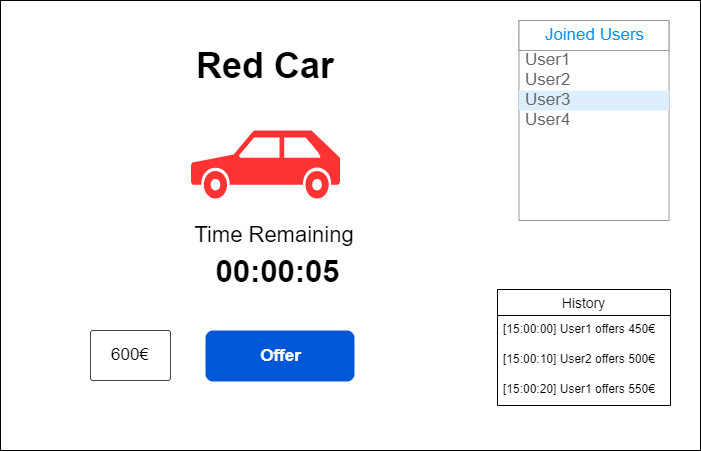
\includegraphics[width=0.7\linewidth]{img/wireframeDSMT.drawio}
	\caption{Mockup of the main interface}
	\label{fig:wireframedsmt}
\end{figure}

\subsection{Design Ideas}
We were thinking of implementing the system in the following way, following a 3-tier architecture:
\begin{itemize}
	\item \textbf{Presentation Tier}: User Interface via HTML/CSS, generated via Java Servlets and JSP
	\item \textbf{Business Logic}: consists of data synchronization on nodes (information to synchronize regards the remaining time of an auction, joined users of an auction, auction history, list of available auctions) and auction winner election
	\item \textbf{Data Access/Storage}: through Erlang by using Mnesia
\end{itemize}